\documentclass[11pt]{article}
\usepackage[a4paper,margin=1in]{geometry}
\usepackage{graphicx}
\usepackage{booktabs}
\usepackage{siunitx}
\usepackage{hyperref}
\title{Vertical Aerosol Confinement and UV Attenuation in the UTLS: A Minimal High‑Altitude Balloon Profiling Case Study over Semi‑Arid Northern India}
\author{Archana Radhakrishnan\thanks{Independent researcher, India.\email{anju.archana@gmail.com}} \and Mani~J.\thanks{Indian Institute of Remote Sensing (IIRS), Indian Space Research Organisation (ISRO), Dehradun, India.\email{mani.joe.thoppil@gmail.com}} \and Bosco\thanks{Independent researcher, India.\email{bosco8b4824@gmail.com}}}
\date{}

\begin{document}
\maketitle

\begin{abstract}
This paper documents a minimal, methods‑focused high‑altitude balloon profiling case study over semi‑arid northern India.  A broadband ultraviolet sensor is used strictly as a relative intensity proxy for aerosol attenuation, and a pressure sensor provides the vertical coordinate.  The executed analysis retained 92 quality‑controlled altitude bins (from 1,444 raw rows, binned into 111 rows) and reached a peak altitude of \SI{17,507.5}{m} at launch coordinates \SI{25.29785}{\degree}~N, \SI{76.19183}{\degree}~E (launch on 5~October~2025 at 07:40~IST).  Across the retained ascent, solar zenith angle (SZA) varied from \SI{45.33}{\degree} to \SI{77.50}{\degree} (median \SI{57.88}{\degree}) and relative airmass $m$ from 1.42 to 4.53 (median 1.88).  The canonical ground‑proxy aerosol optical depth was $\tau_{\mathrm{aer}}=0.1054$; confinement heights defined by cumulative optical depth were $z_{50}=\SI{10,721.81}{m}$ and $z_{90}=\SI{2,776.83}{m}$.  Satellite aerosol optical depth (AOD) was used for comparison only; the high‑altitude balloon profile is the primary dataset.
\end{abstract}

\section{Introduction}
Vertical structure of aerosols in the upper troposphere and lower stratosphere (UTLS) influences radiative transfer and informs the interpretation of satellite column retrievals.  Satellite products offer broad spatial coverage but limited vertical resolution.  Balloon‑borne profiles provide valuable high‑vertical‑resolution reference data for closure studies.  This work presents a minimal case study: a single high‑altitude balloon flight using a broadband ultraviolet radiometer as a relative optical proxy and a pressure sensor for altitude estimation.  The emphasis is on transparency and reproducibility; all quantitative results reported in this manuscript are reproduced directly from the executed analysis.

\section{Materials and Methods}

\subsection{Instrumentation}
Two sensors form the core of the payload (Table~\ref{tab:sensors}).  The ultraviolet channel is an Apogee SU‑200/202 class radiometer used strictly as a relative intensity proxy.  Manufacturer documentation lists a spectral response spanning \SI{305}{\nano\metre}--\SI{390}{\nano\metre} (response $>$\SI{10}{\percent} of peak) with a hemispherical field of view (180\,\degree).  Output sensitivity is \SI{25}{mV~(W\,m^{-2})^{-1}}; equivalently, the reciprocal calibration factor is \SI{0.04}{W~m^{-2}~mV^{-1}}.  Calibration uncertainty is stated as \(\pm 5\,\%\), and long‑term drift is less than \SI{2}{\percent} per year.  The sensor is calibrated traceably to NIST.  A larger dynamic‑range variant (SU‑200) yields \SI{10}{\milli\volt} at \SI{1}{W~m^{-2}} and is included in Table~\ref{tab:sensors} for completeness; however, the present flight uses the amplified SU‑202 model.  The pressure sensor is a Bosch BME280 environmental module measuring pressure, temperature and humidity.  Documentation lists an operating pressure range of \SIrange{300}{1100}{hPa} with absolute accuracy around \SI{1}{hPa} and relative accuracy of \SI{0.12}{hPa}.  These specifications support altitude estimation via the hypsometric equation.

\begin{table}[h]
\centering
\caption{In‑scope sensors and key manufacturer specifications.  Only values explicitly provided in datasheets are listed.}
\label{tab:sensors}
\begin{tabular}{@{}lll@{}}
\toprule
Sensor & Measured quantity & Key specifications \\ \midrule
Apogee SU‑202 (UV radiometer) & Relative ultraviolet irradiance (proxy) & Spectral range \SI{305}{--}\SI{390}{nm}; 180\,\degree field of view; sensitivity \SI{25}{mV~(W\,m^{-2})^{-1}}; calibration uncertainty \(\pm 5\,\%\); long‑term drift $<$\SI{2}{\percent}\,yr$^{-1}$; NIST traceable calibration. \\ \addlinespace
Apogee SU‑200 (reference model) & Same quantity (lower gain) & Output \SI{10}{\milli\volt} per \SI{1}{W~m^{-2}}; calibration factor \SI{10}{W~m^{-2}~mV^{-1}}; calibration uncertainty \(\pm 5\,\%\); spectral range \SI{305}{--}\SI{390}{nm}. \\ \addlinespace
Bosch BME280 & Pressure; temperature; humidity & Pressure range \SIrange{300}{1100}{hPa}; absolute accuracy $\approx$\SI{1}{hPa}; relative accuracy \SI{0.12}{hPa}; operating temperature range \SI{-40}{\degree C}--\SI{85}{\degree C}. \\ \bottomrule
\end{tabular}
\end{table}

\subsection{Data processing and quality control}
The analysis pipeline ingests 1,444 raw rows and bins them into 111 altitude segments.  Quality‑control (QC) filters exclude bins with saturation/floor behaviour or unstable vertical gradients, retaining 92 bins (\SI{82.9}{\percent} of binned data).  Figure~\ref{fig:qc} visualises QC acceptance.  The ultraviolet proxy is treated strictly as a relative intensity; an uncertainty of 10~\% is assigned to account for sensor drift and residual calibration factors.

\subsection{Solar geometry and airmass correction}
Solar zenith angle $z$ is computed from latitude, longitude and UTC time using NOAA‑style solar position equations.  Relative airmass $m$ is calculated from $z$ using the Kasten–Young approximation:
\begin{equation}
m = \frac{1}{\cos z + 0.50572\,(96.07995 - z)^{-1.6364}},
\end{equation}
subject to caps $z\leq \SI{85}{\degree}$ and $m \leq 10$.  The executed run reports SZA spanning \SI{45.33}{\degree} to \SI{77.50}{\degree} and airmass between 1.42 and 4.53.

\subsection{Optical proxy retrieval and confinement metrics}
The broadband UV intensity $I(z)$ is converted to a proxy optical depth profile via
\begin{equation}
\tau_{\mathrm{eff}}(z) = \frac{\ln\left(I_{\mathrm{top}}/I(z)\right)}{m},
\end{equation}
where $I_{\mathrm{top}}$ is a top‑of‑profile reference intensity and $m$ is airmass.  Rayleigh attenuation is estimated from pressure (and an assumed effective wavelength) and subtracted to obtain an aerosol proxy $\tau_{\mathrm{aer}}(z)=\max(\tau_{\mathrm{eff}}(z) - \tau_{\mathrm{Rayleigh}}(z), 0)$.  A canonical near‑surface proxy value $\tau_{\mathrm{aer}}(z_{\mathrm{ref}})=0.1054$ is reported.  The cumulative fraction of total column proxy above altitude $z$ is used to define confinement scales: $z_{50}$ and $z_{90}$ are the minimum altitudes at which the cumulative proxy drops below 50\,\% and 10\,\% of the surface value, respectively.  For this flight $z_{50}=\SI{10,721.81}{m}$ and $z_{90}=\SI{2,776.83}{m}$.

\section{Results}
\subsection{Run summary}
Table~\ref{tab:summary} lists key metrics reproduced directly from the executed analysis.  The peak altitude was \SI{17,507.5}{m}.  Solar zenith angle and airmass ranges reflect the changing geometry during ascent.  The quality‑controlled dataset retained 92 of 111 binned rows.  Canonical aerosol proxy and confinement scales are as described above.

\begin{table}[h]
\centering
\caption{Run summary metrics from the executed analysis.}
\label{tab:summary}
\begin{tabular}{@{}ll@{}}
\toprule
Metric & Value \\ \midrule
Raw rows / binned rows / QC‑retained rows & $1{,}444 / 111 / 92$ \\ 
Peak altitude & \SI{17,507.5}{m} \\ 
Solar zenith angle (min / median / max) & \SI{45.33}{\degree} / \SI{57.88}{\degree} / \SI{77.50}{\degree} \\ 
Airmass (min / median / max) & 1.42 / 1.88 / 4.53 \\ 
Canonical $\tau_{\mathrm{aer}}$ (ground proxy) & 0.1054 \\ 
Confinement scales & $z_{50}=\SI{10,721.81}{m}$, $z_{90}=\SI{2,776.83}{m}$ \\ 
\bottomrule
\end{tabular}
\end{table}

\subsection{Figures}
Figures~\ref{fig:proxy}–\ref{fig:segment} reproduce the diagnostics produced by the executed run.  Figure~\ref{fig:proxy} shows the relative intensity proxy as a function of altitude.  Figure~\ref{fig:qc} visualises quality‑control acceptance and rejection.  Figure~\ref{fig:sanity} displays sensor sanity checks (proxy versus temperature and time).  Figure~\ref{fig:sat} shows saturation/floor detection.  Figure~\ref{fig:segment} illustrates segment‑consistency for $\tau_{\mathrm{aer}}(z)$ across different top‑of‑profile selections.

\begin{figure}[h]
\centering
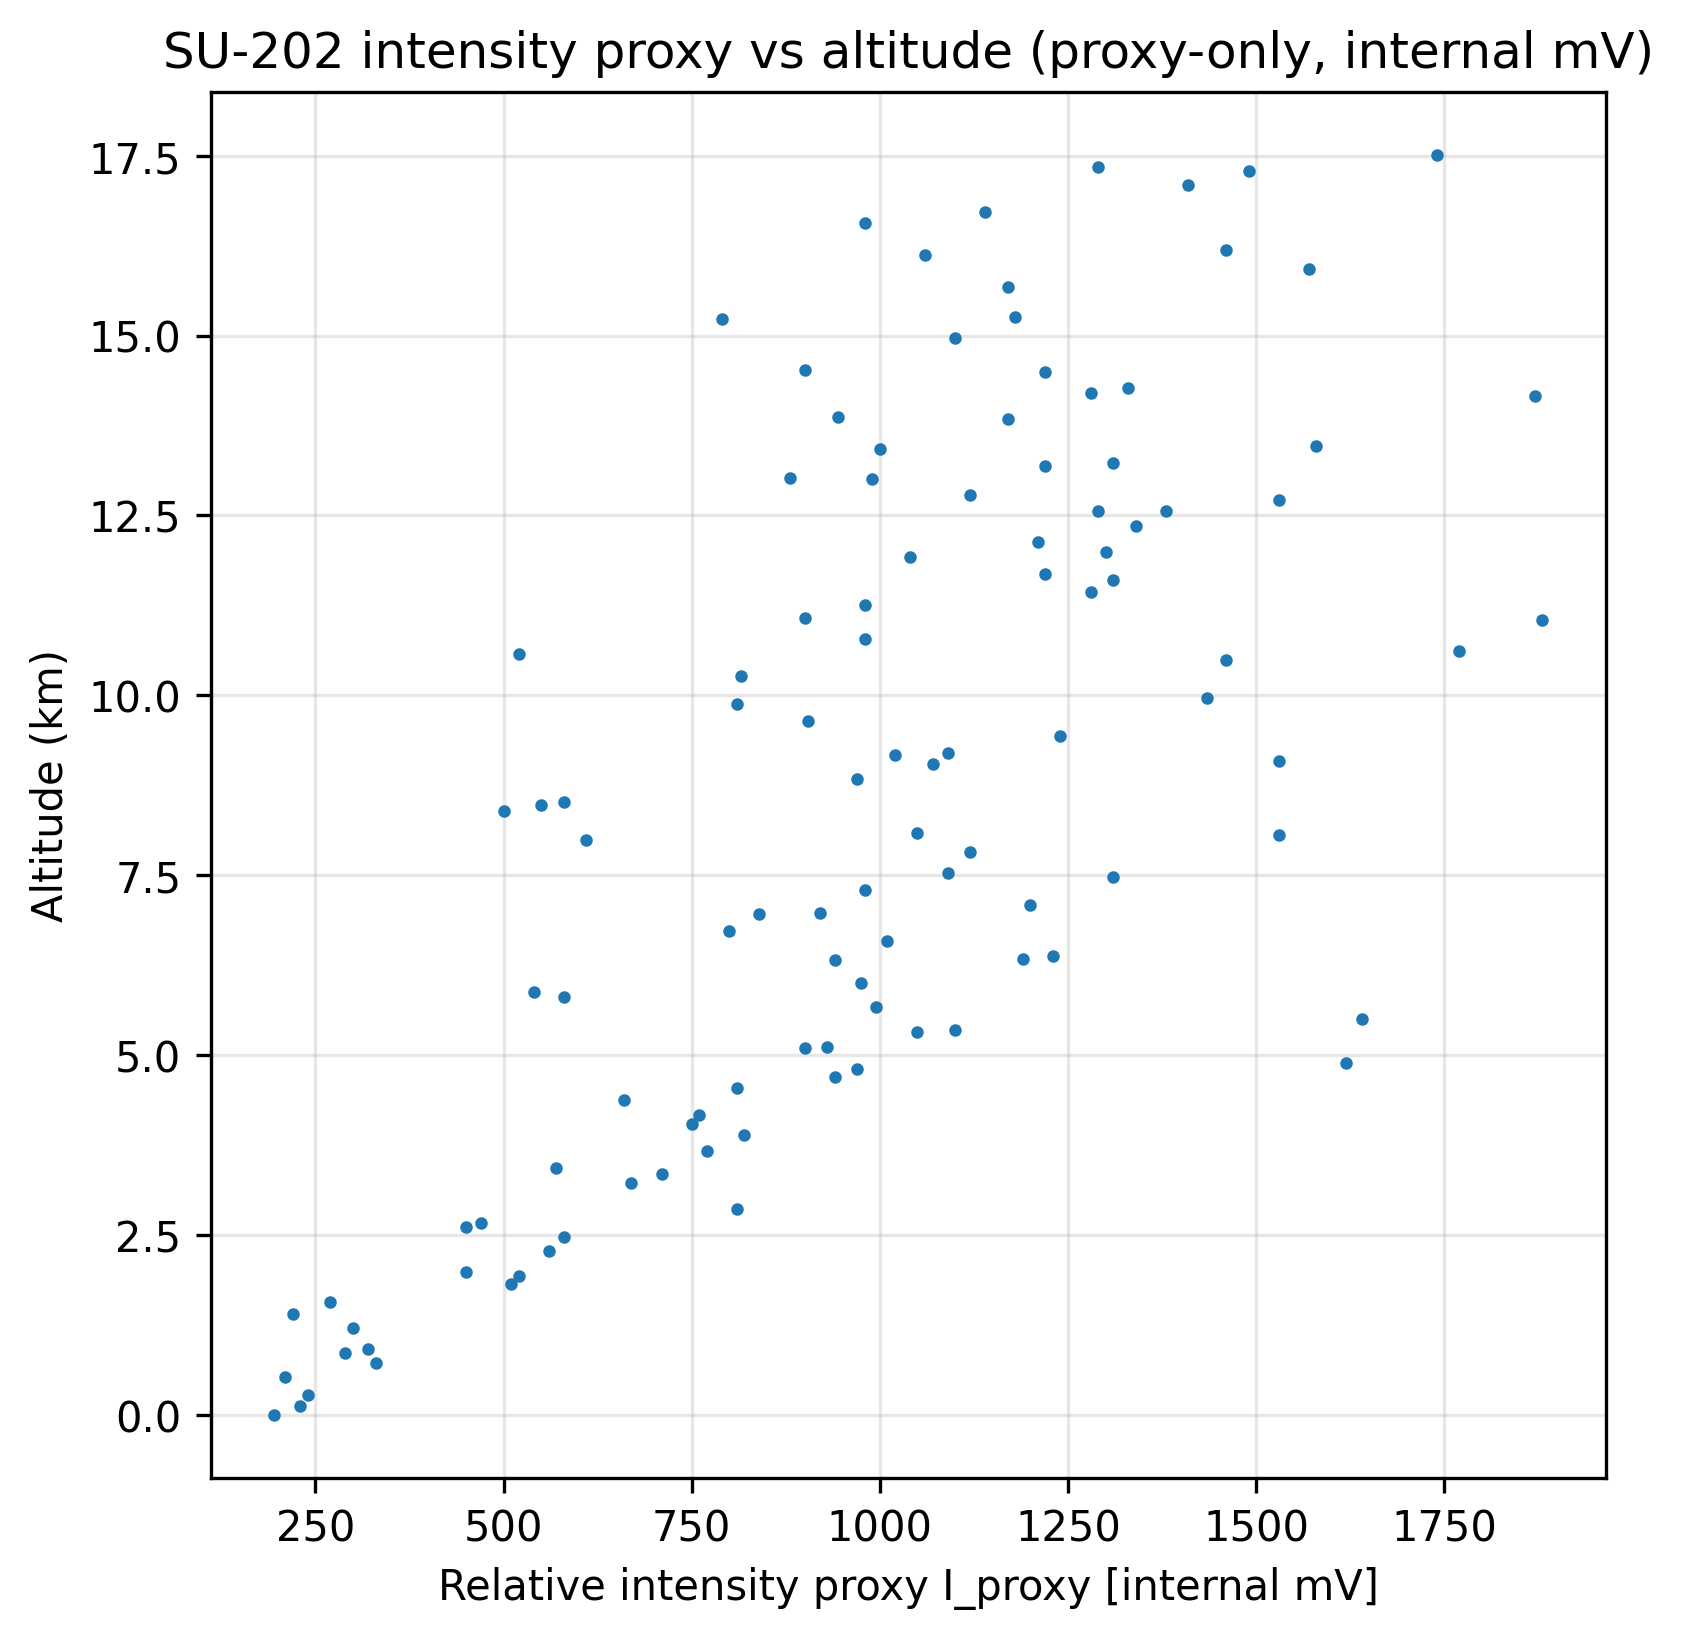
\includegraphics[width=0.9\textwidth]{figures/Fig01_su202_proxy_vs_alt.png}
\caption{Relative SU‑202 intensity proxy vs altitude.  Values are internal millivolts; no radiometric conversion is applied.}
\label{fig:proxy}
\end{figure}

\begin{figure}[h]
\centering
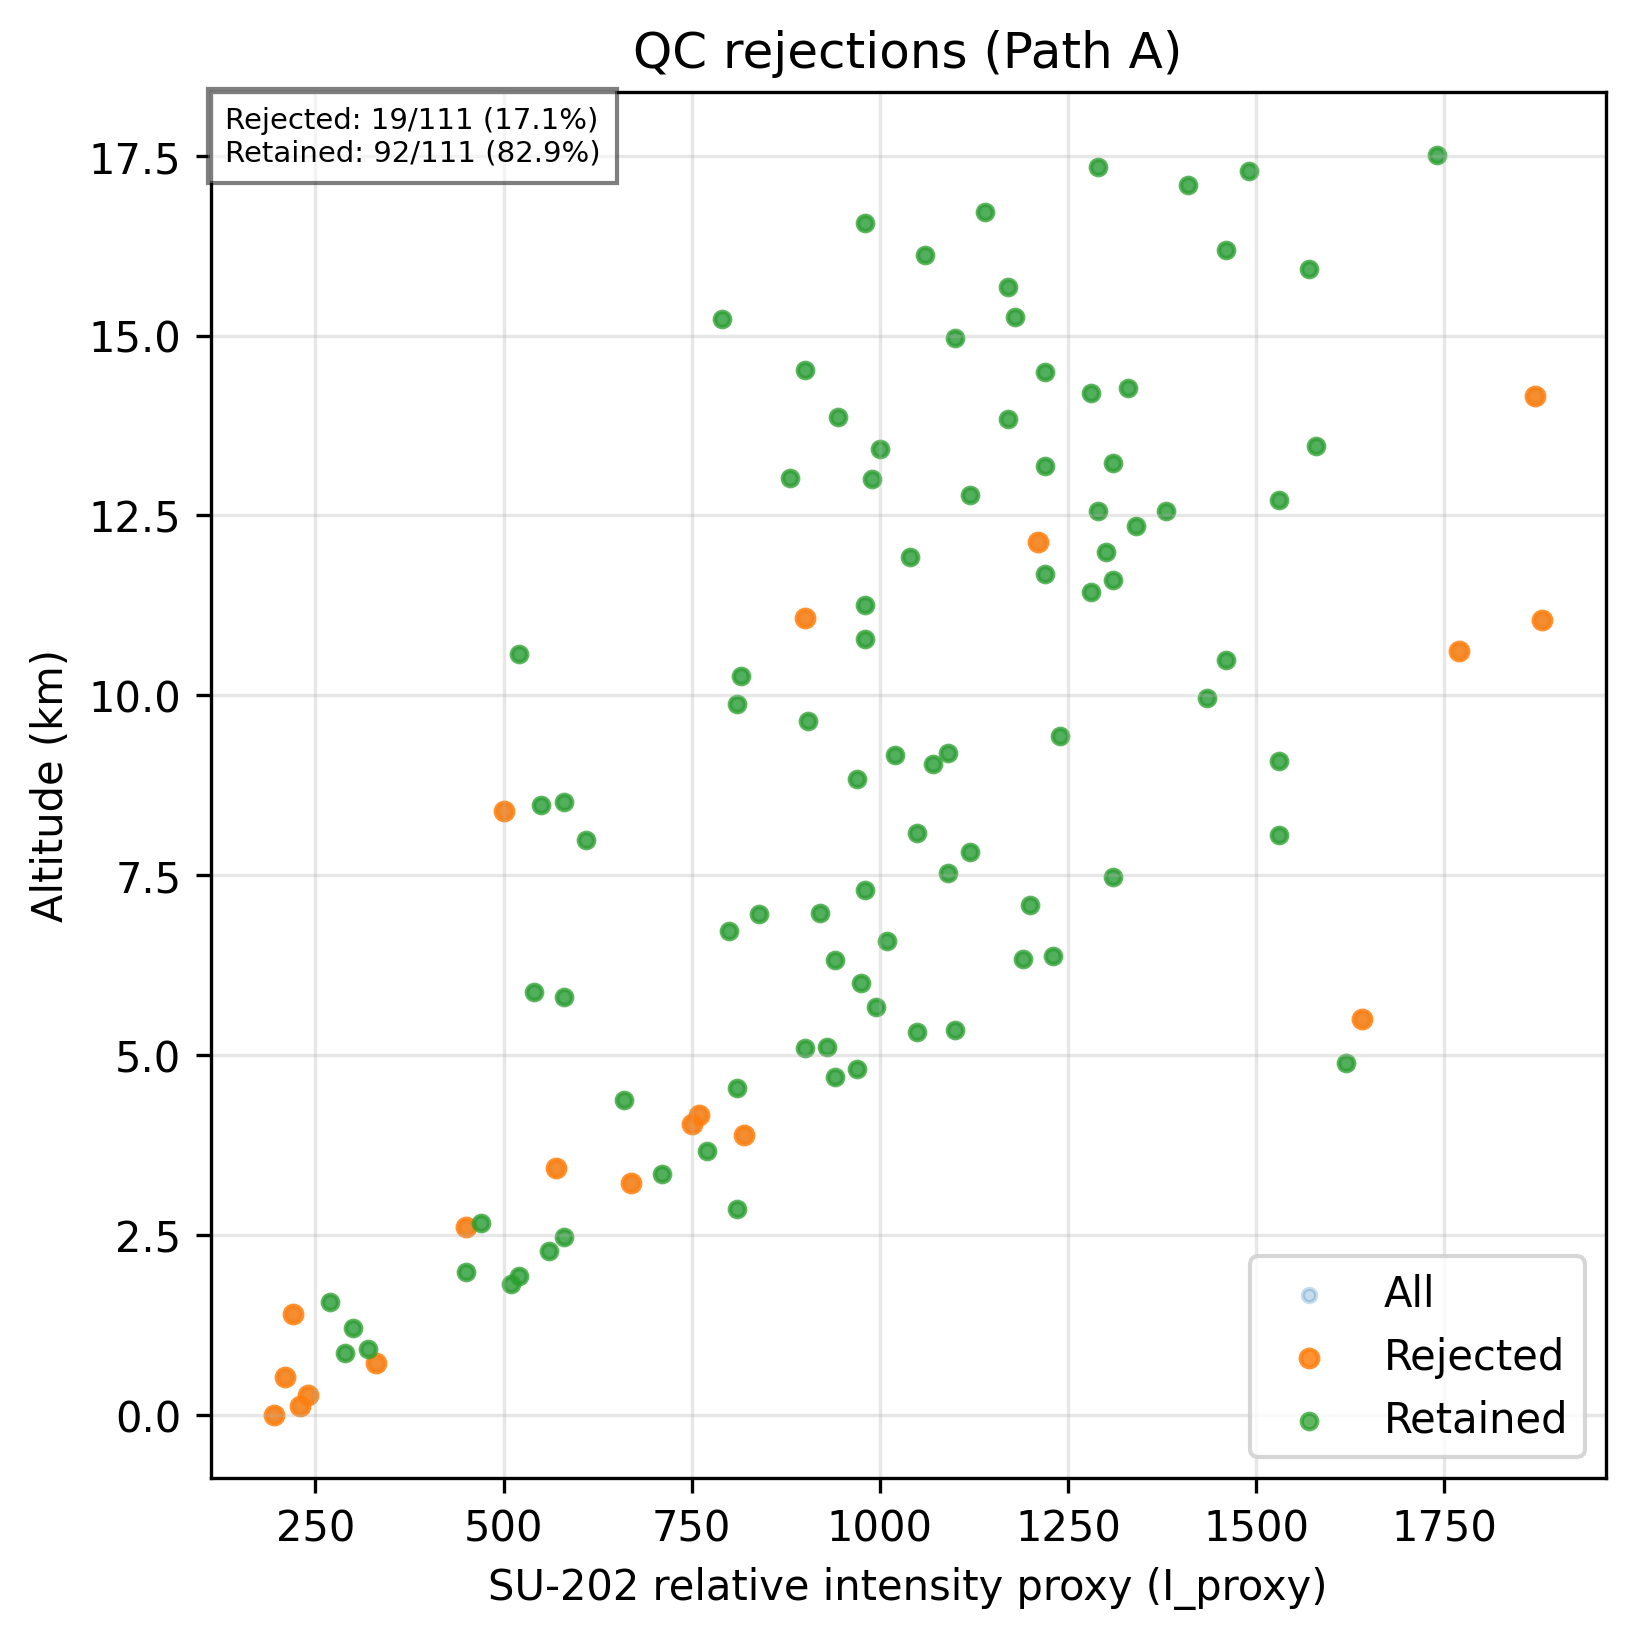
\includegraphics[width=0.9\textwidth]{figures/Fig02_qc_rejections.png}
\caption{Quality control rejections and retained bins.  Green indicates retained bins; orange indicates rejected bins.}
\label{fig:qc}
\end{figure}

\begin{figure}[h]
\centering
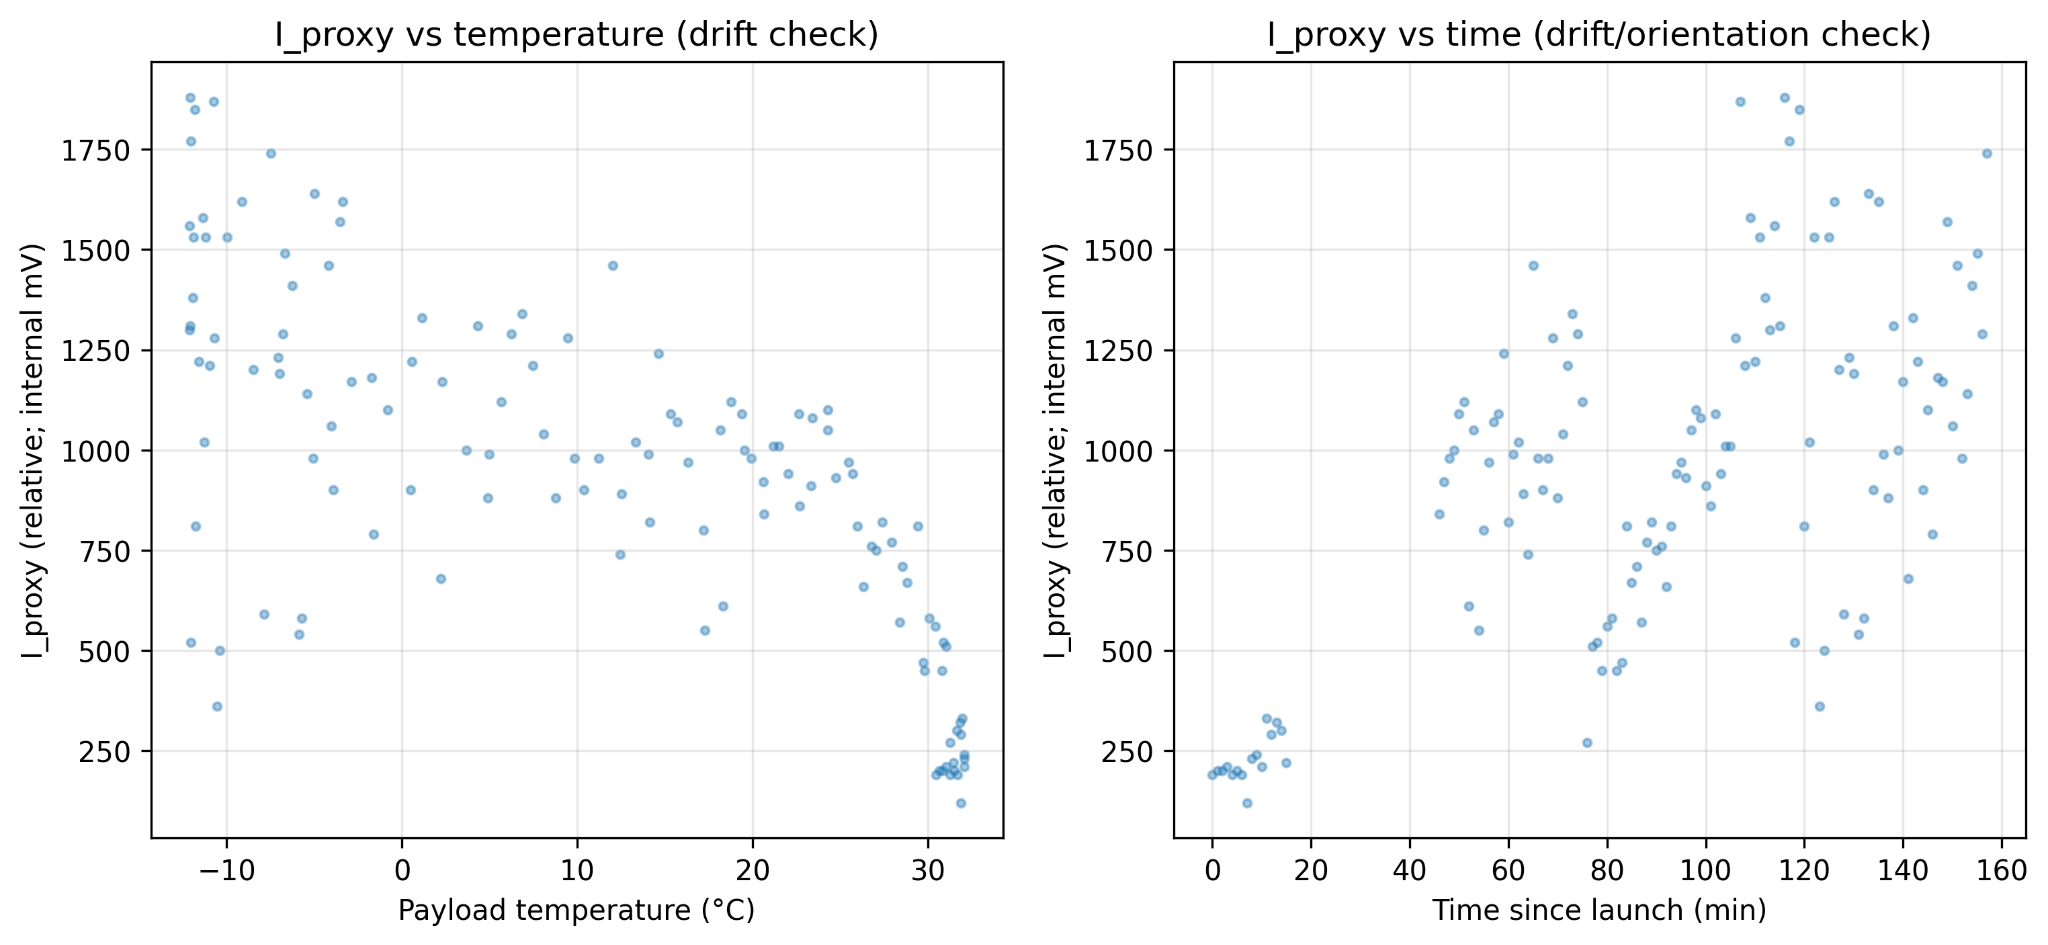
\includegraphics[width=0.9\textwidth]{figures/Fig06_sensor_sanity.png}
\caption{Sensor sanity diagnostics: proxy vs temperature (left) and proxy vs time since launch (right).  These checks ensure no strong drift or orientation effects.}
\label{fig:sanity}
\end{figure}

\begin{figure}[h]
\centering
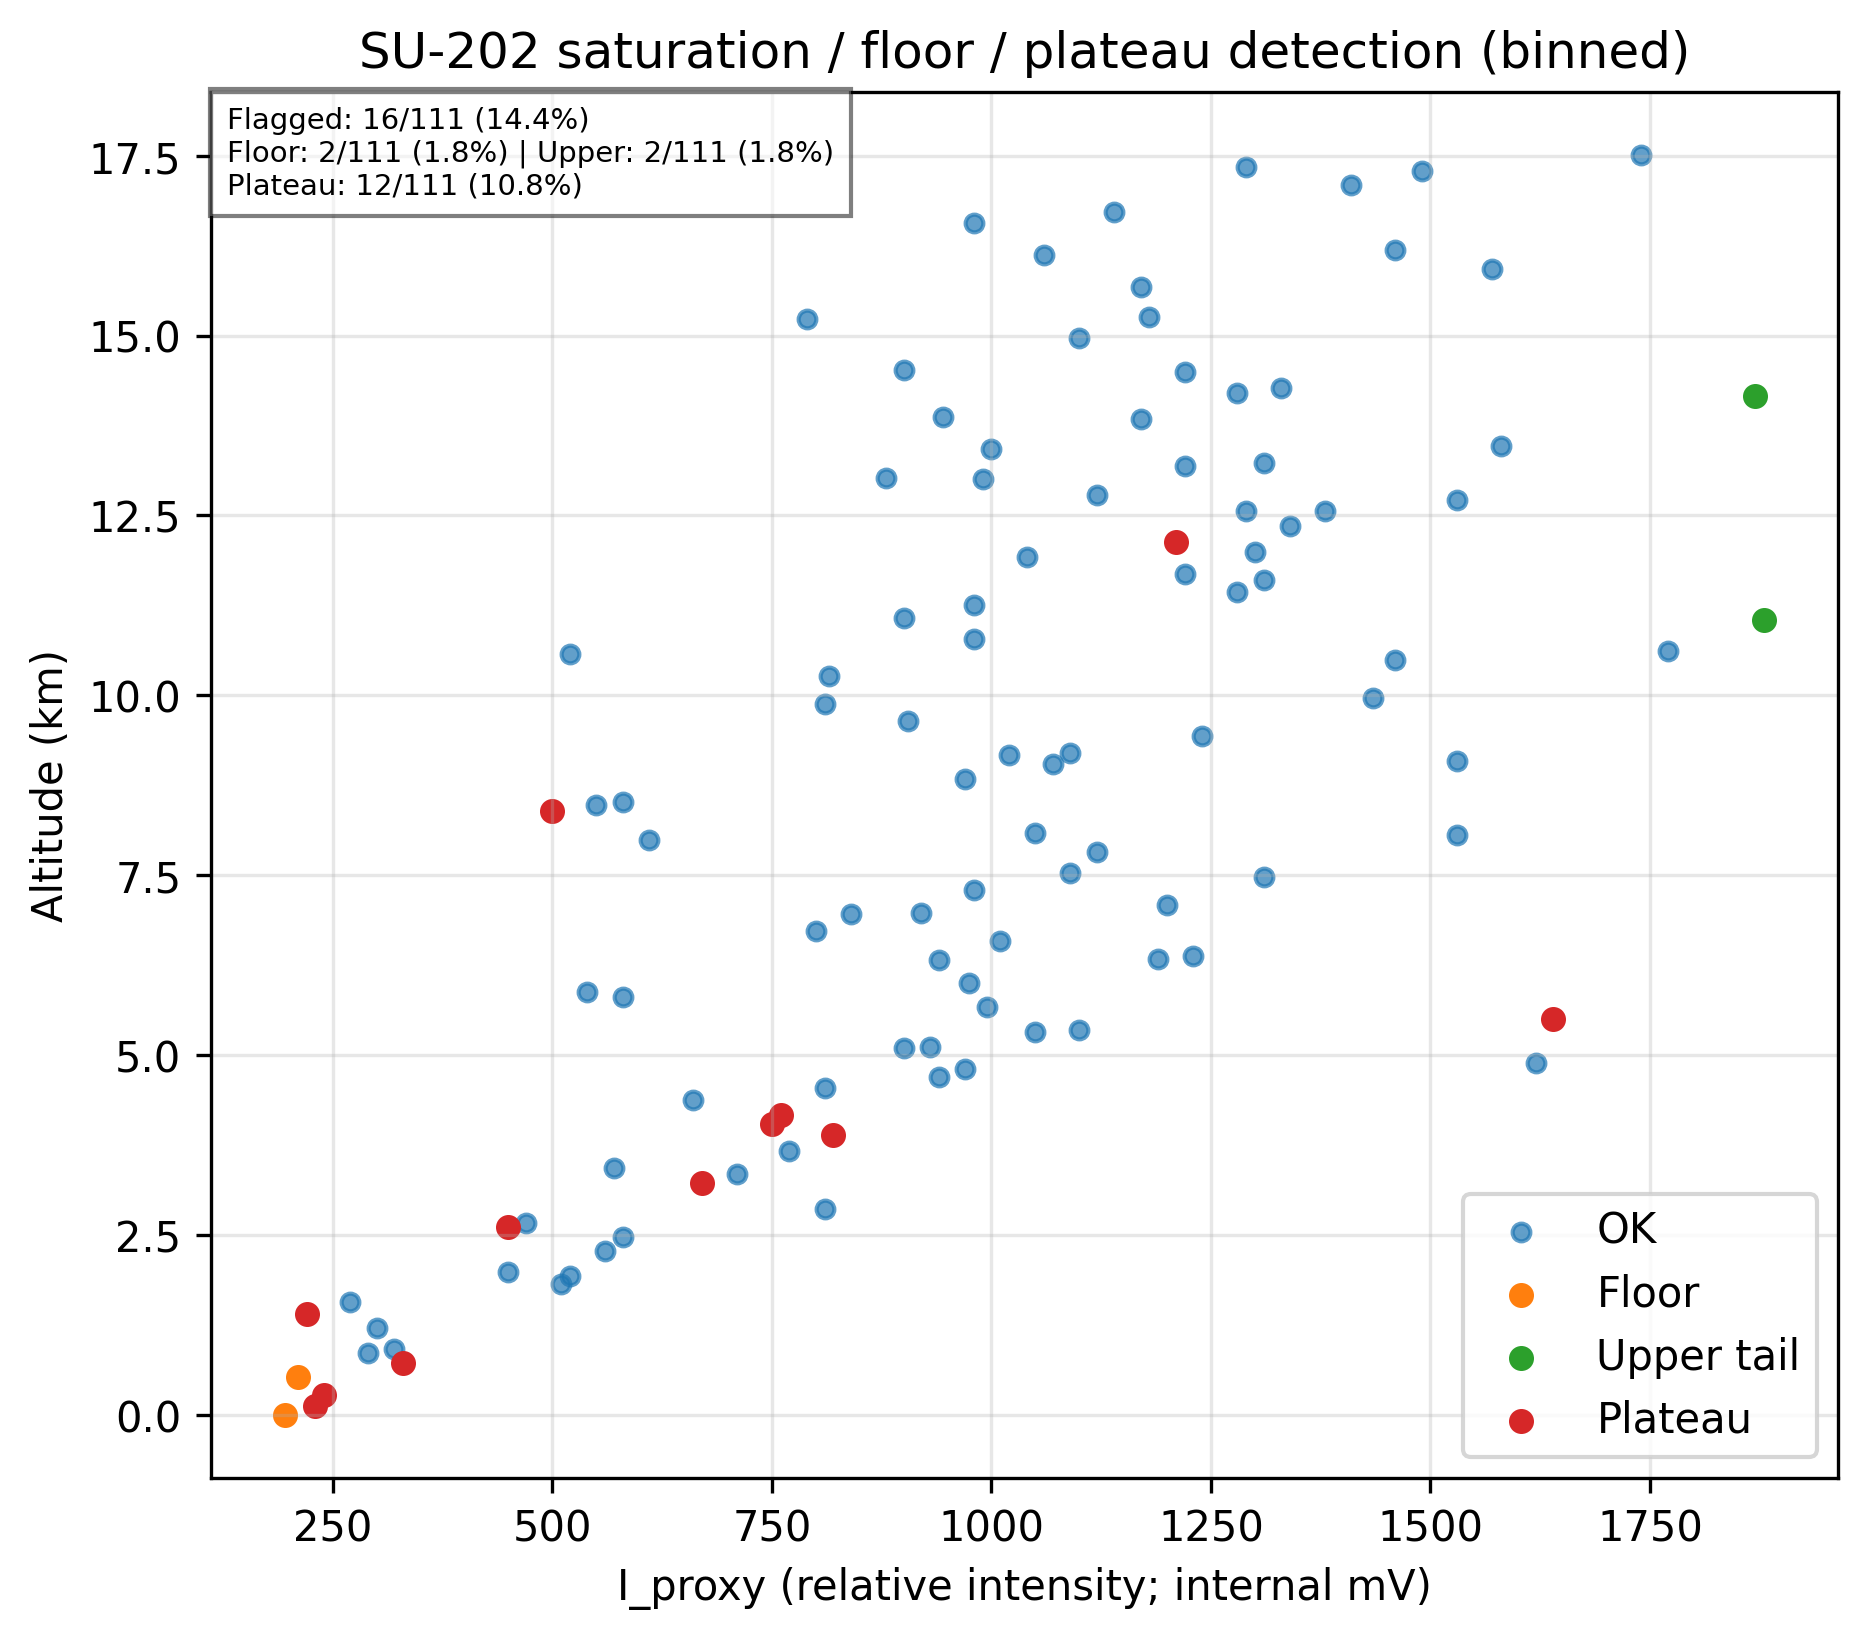
\includegraphics[width=0.9\textwidth]{figures/Fig09_saturation_floor_detection.png}
\caption{Saturation, floor and plateau detection for the SU‑202 proxy.  Points flagged as plateau or saturation are excluded by QC.}
\label{fig:sat}
\end{figure}

\begin{figure}[h]
\centering
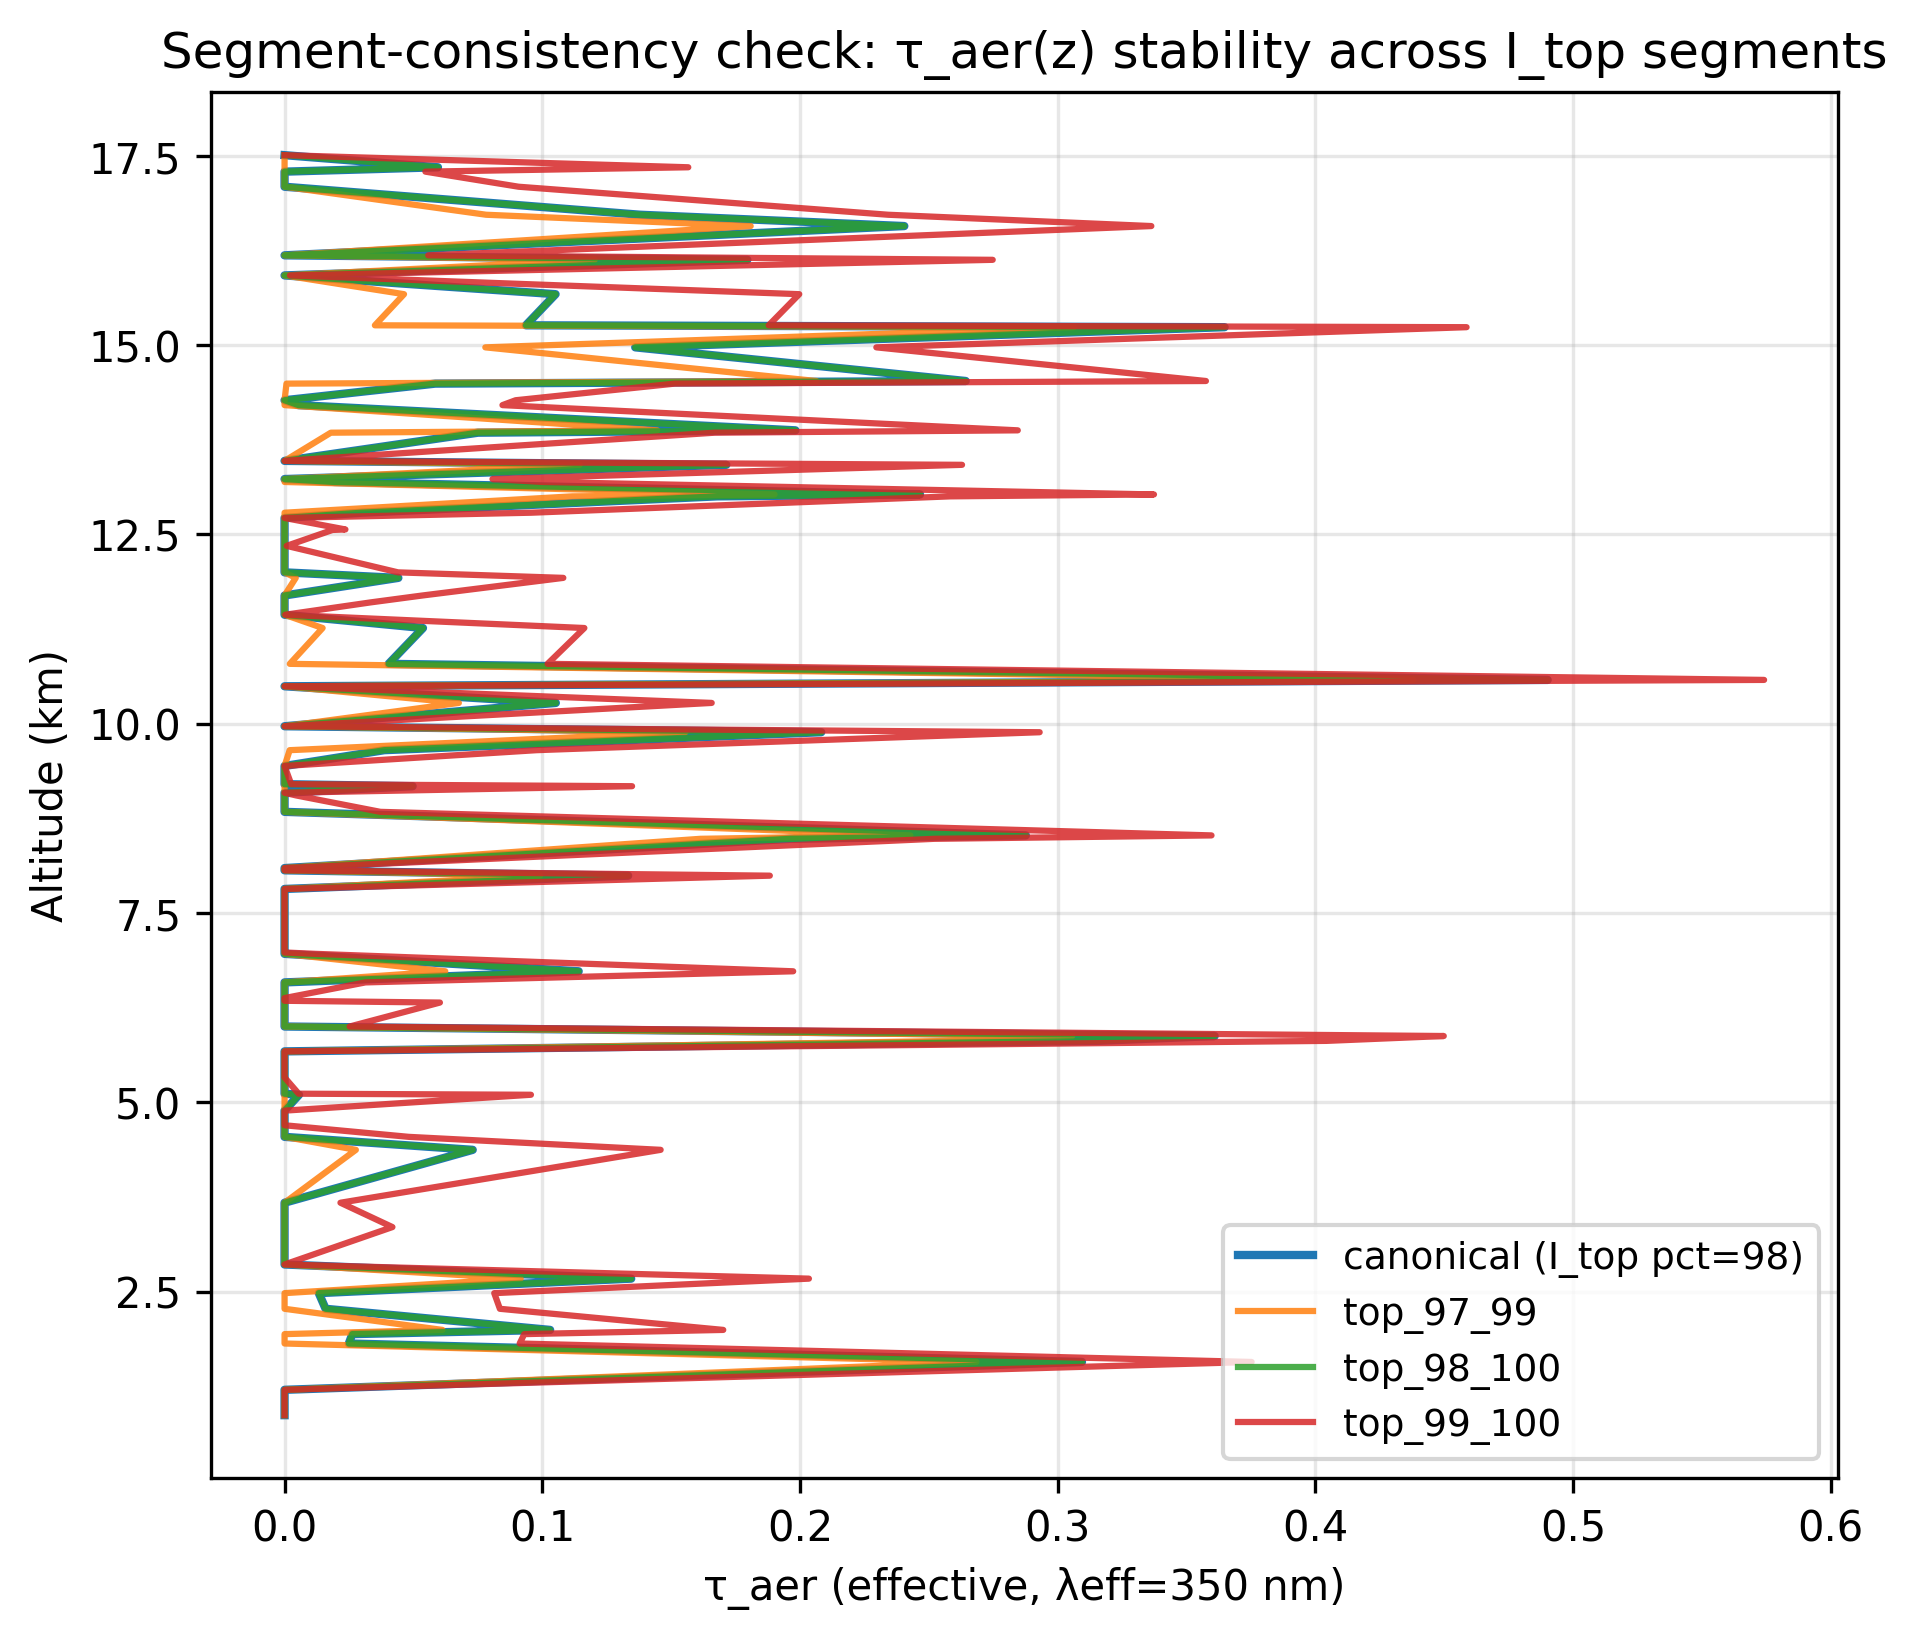
\includegraphics[width=0.9\textwidth]{figures/Fig10_tau_segment_consistency.png}
\caption{Segment‑consistency check: stability of $\tau_{\mathrm{aer}}(z)$ across alternative top‑of‑profile definitions.  Curves correspond to different top percentile intervals.  Consistency across curves supports robustness.}
\label{fig:segment}
\end{figure}

\section{Data and Code Availability}
All data, figures, and the executed notebook underlying this study are archived in a Zenodo repository (DOI to be assigned).  The dataset includes the processed high‑altitude balloon measurements (\texttt{datalog\_cleaned\_with\_altitude.csv}), satellite comparison files (if used), the Jupyter notebook \texttt{EarthArXiv\_final\_clean2\_run\_2025-10-05.ipynb}, the executed HTML report \texttt{eartharxiv\_clean2\_new\_run\_fixed.html}, and all figure PNGs.  Sensor specification PDFs are provided for transparency.  The GitHub repository hosting the manuscript, notebook, and analysis scripts is publicly available; the Zenodo deposit archives the exact release corresponding to this manuscript.

\section{Conclusion}
A single high‑altitude balloon flight provided a reproducible profile of relative UV attenuation in the UTLS over semi‑arid northern India.  Pressure‑derived altitude, solar‑geometry correction and proxy‑only retrieval yielded a canonical near‑surface aerosol optical depth and confinement scales.  All reported metrics are reproducible from the published notebook and data.  The case study emphasises methodological transparency rather than novelty; the presented workflow can serve as a template for future low‑cost high‑altitude profiling experiments.

\end{document}